
\chapter{Modelling with XML Data}

There is a general requirement for model data to be interchangeable
between tools. This is because organisations rely increasingly on
tool chains to support their business. No single tool can support
the whole process. Data generated by a modelling tool might hand the
information on to a code-generation tool or might hand the information
on to an engine that runs the models directly. In any case the different
tools in the tool chain need to agree on a format for the data.

In order to have different tools work with shared data there needs
to be a common serialization format. Data is serialized when it is
exported into a format that can be saved in a file. The format of
the data in the file needs to be known to all tools in the chain.
The format definition is often referred to as \textit{meta-data.}

The de-facto standard for data representation is XML. It is a textual
format that can be saved to files. Essentially, XML data is a tree
where each node in the tree is either raw text or is an element. An
element has a tag and some name/value attribute pairs. Each element
has a sequence of child nodes. Often you can think of the node tag
as the type of the node (for example: an employee record or a customer
transaction) and the attribute pairs as containing node properties
(for example: the employee name or the date of the transaction). The
children of the node usually encode relationships (for example: employee-to-department
or transaction-to-product).

XML meta-data (often also encoded as XML) defines the legal structure
of the XML documents. For example it defines the set of tags that
can be used in elements, the legal set of attributes for an element
with a given tag and the order in which child nodes can occur.

Both models and model instance data can be encoded using XML. For
example, the UML modelling language has an XML meta-data definition
called XMI that defines how UML models are serialized and therefore
shared between UML tools. 

When using a model-driven approach to system development it is important
to understand how to serialize and de-serialize model data. You may
be using a standard meta-data definition or be designing one of your
own. This chapter describes a number of language driven approaches
to using XML data.

%
\begin{figure}
\begin{center}

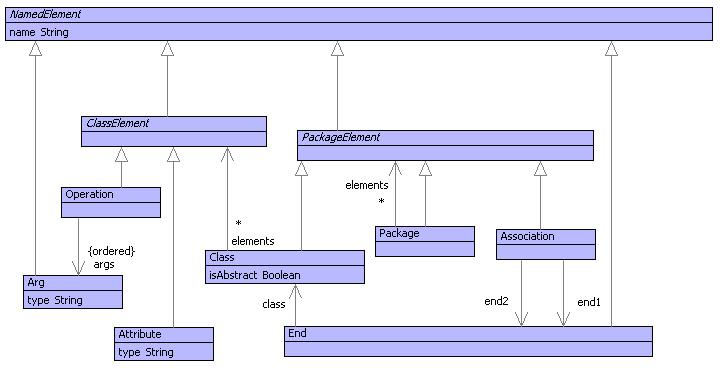
\includegraphics[width=12cm]{LanguageEngineering/XML/Images/Models}
\caption{Models\label{fig:Models}}

\end{center}
\end{figure}


Figure \ref{fig:Models} shows a simple UML-style modelling language
consisting of packages of classes and associations between them. This
chapter shows how instances of this language can be serialized as
XML data and how the resulting files can be read back into models.


\section{Generating XML Data}

Given an instance of the modelling language defined in figure \ref{fig:Models},
the translation to XML data is straightforward. Each class defines
an operation toXML that takes an output channel to which XML is written.
The format of XML data is standard, so it is useful to define a language
construct to support its generation. The following shows how the toXML
operation for Package is defined:

\begin{lstlisting}
@Operation toXML(out:OutputChannel)
  @XML(out)
    <Package name=self.name>
      @For e in elements do
        e.toXML(out)
      end
    </Package>
 end
end
\end{lstlisting}The XML construct is used to guide the generation of XML data to an
output channel. The output channel is supplied in ( and ) after @XML.
The body of the @XML construct defines the format of the generated
XML data. An XML element has the format:

\begin{lstlisting}
<TAG ATTS>
  CHILDREN
</TAG>
\end{lstlisting}where TAG is just a name, ATTS is a sequence of attribute value pairs,
CHILDREN is a sequence of child nodes and the final </TAG> should
match up with the corresponding opening tag. In the example, the tag
is Package, there is a single attribute called name. The value of
the name attribute (on the right of the =) is the name of the package. 

The @XML language construct allows XML elements to be written as they
will appear in the output, the characters will be send to the supplied
output channel. This makes it easy for the system to check that there
are no mistakes in the XML format and removes the need for the user
to have to use a format-statement or equivalent to describe how the
output should appear.

The children part of the @XML construct for packages is an XOCL @For
statement that iterates through the package elements and invokes their
toXML operations, supplying the same output channel.

%
\begin{figure}
\begin{center}

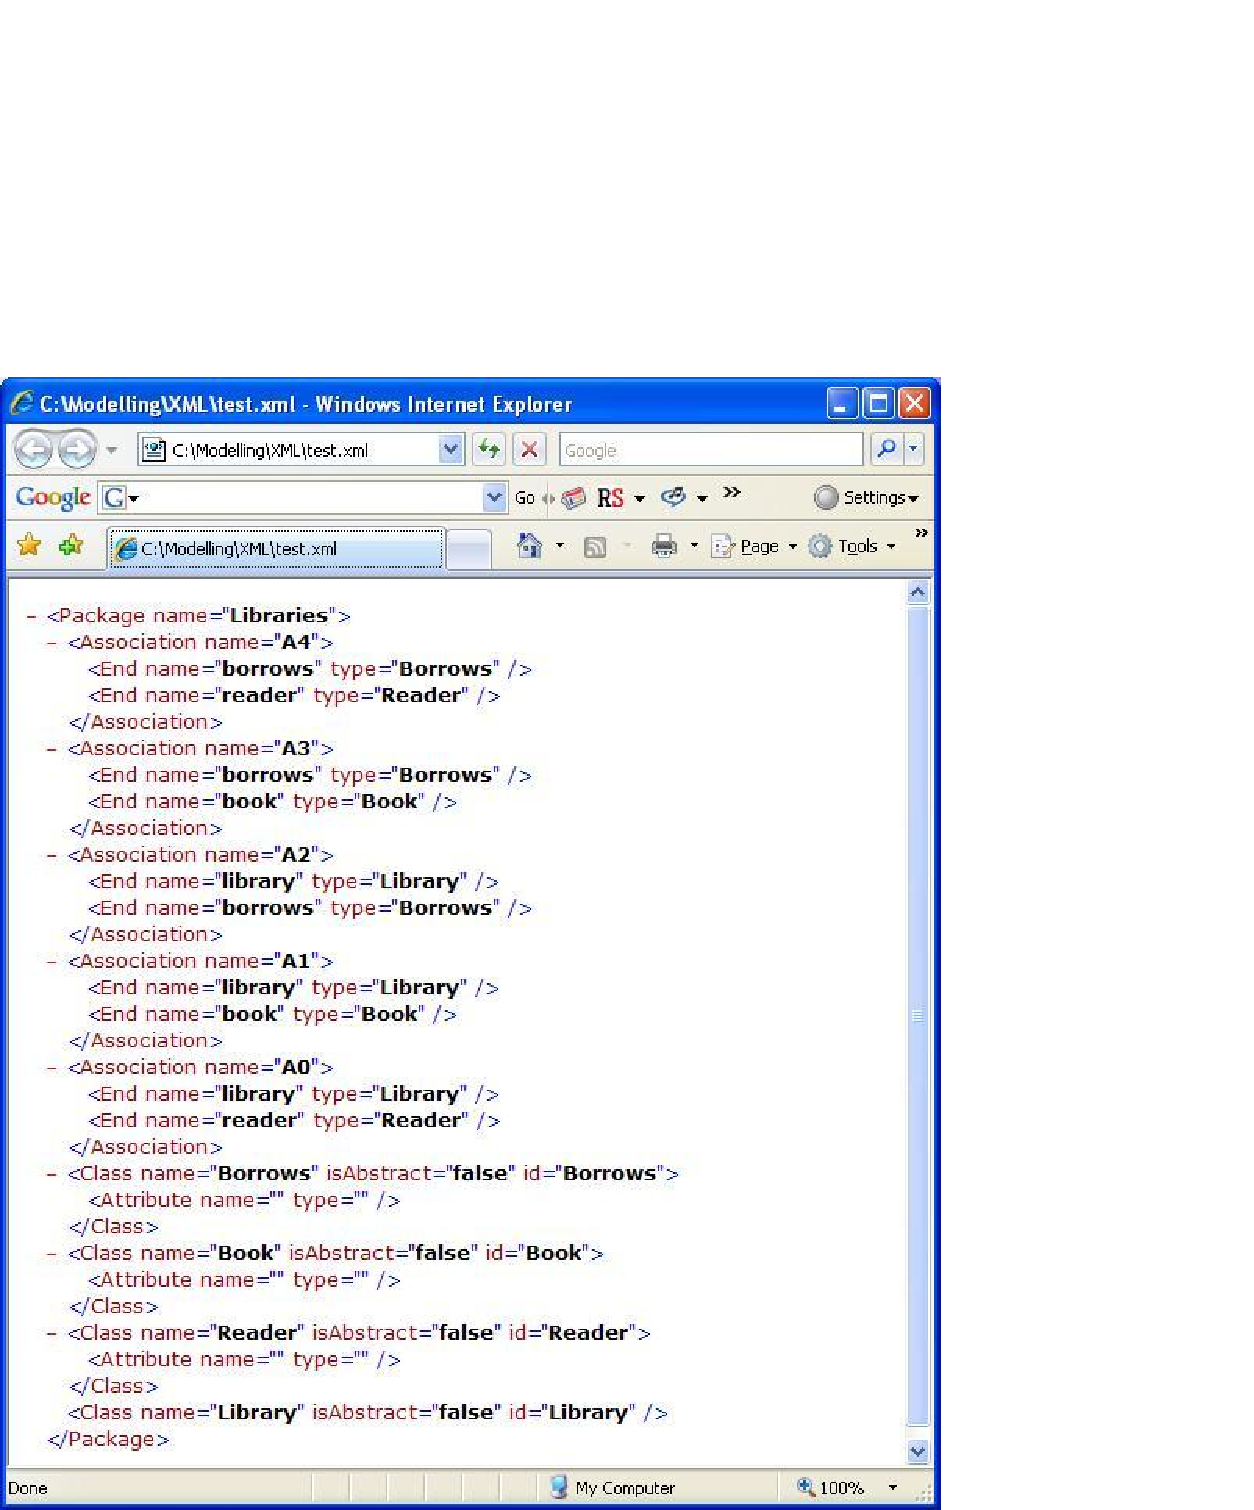
\includegraphics[width=12cm]{LanguageEngineering/XML/Images/Libraries}

\caption{A Simple Model Serialized as XML\label{fig:A-Simple-Model-as-XML}}

\end{center}
\end{figure}


Figure \ref{fig:A-Simple-Model-as-XML} shows a simple library model
serialized as XML using the toXML operations. Notice that the classes
attached to the ends of associations are encoded as the unique identifiers
attributes to the classes (in this case the class names are used as
the class identifiers, however in a real implementation some unique
string is usually used). The rest of this section defines the toXML
operations for all other classes in the modelling language.

Associations just wrap an association element around the two ends:

\begin{lstlisting}
@Operation toXML(out)
  @XML(out)
    <Association name=name>
      end1.toXML(out);
      end2.toXML(out)
    </Association>
  end
end
\end{lstlisting}An end generates a name and an identifier for the class that it attaches
to. The name of the class is used as the identifier:

\begin{lstlisting}
@Operation toXML(out)
  @XML(out)
    <End name=name type=class.name()/>
  end
end
\end{lstlisting}A class generates an element with attributes for the name, whether
it is abstract and its identifier. the children are generated by asking
each element of the class to generate some XML:

\begin{lstlisting}
@Operation toXML(out)
  @XML(out)
    <Class name=name isAbstract=isAbstract id=name>
      @For e in elements do
        e.toXML(out)
      end
    </Class>
  end
end
\end{lstlisting}The toXML operations for attributes, operations and arguments are
very similar to those describes above.


\section{An XML Generator}

The previous section uses a simple language construct to generate
XML output. The language construct allows the output from a model
to be described in XML format rather than using raw character output.
This makes it easier to focus on the structure of the output data
rather than the detail of the XML character formatting. This section
shows how the construct is implemented. 

%
\begin{figure}
\begin{center}

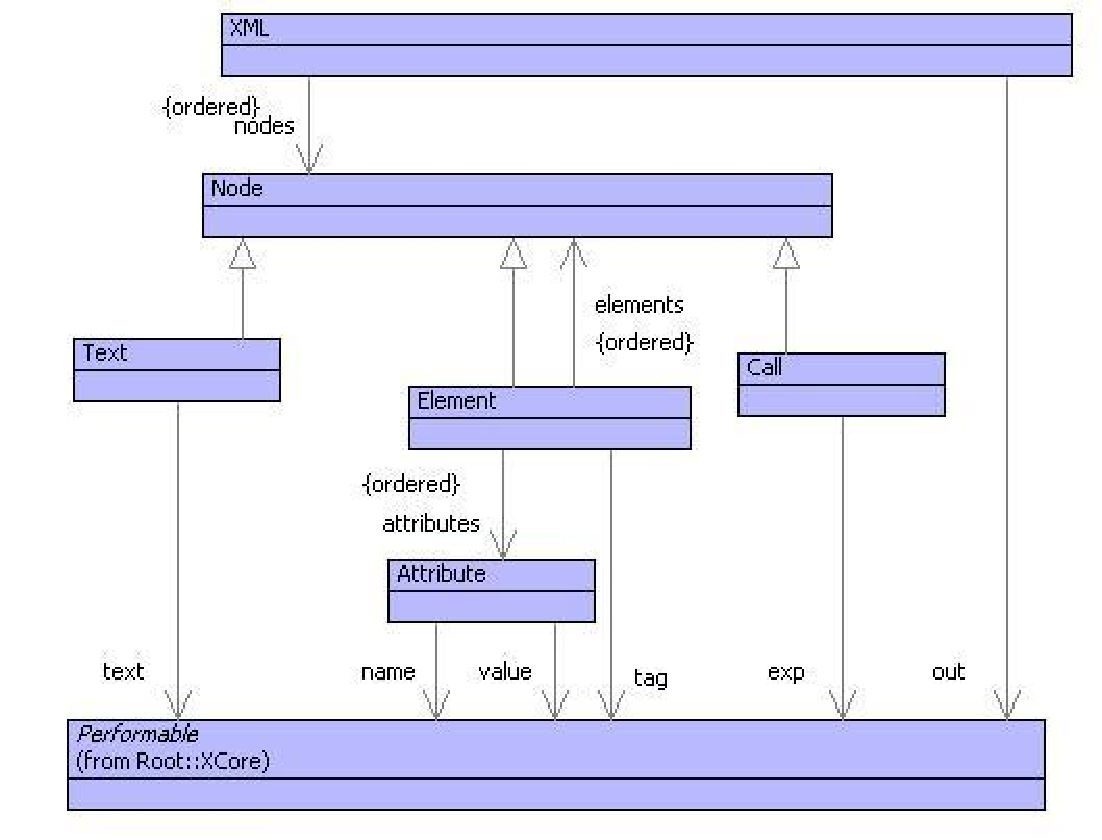
\includegraphics[width=12cm]{LanguageEngineering/XML/Images/PrintXML}

\caption{The PrintXML Classes\label{fig:The-PrintXML-Classes}}

\end{center}
\end{figure}


Figure \ref{fig:The-PrintXML-Classes} shows the classes used to implement
the XML printing construct. An XML template is a performable expression
(out) and a sequence of nodes. The out expression will evaluate to
an output channel at run-time and a node is a syntax construct that
produces XML output to the channel. A text node is an expression that
produces raw text in the XML output. A call node is a general XOCL
expression; this allows any code to be embedded in the XML template
(such as an @For expression). An element is a syntax construct that
formats an XML element to the output channel. The tag and attribute
components are all XOCL expressions that produce strings. An element
node references sub-elements each of which are XML template nodes.

The XML template construct is parsed by the following grammar:

\begin{lstlisting}
@Grammar extends OCL::OCL.grammar
  AtomicElement ::= 
    '<' t = Tag A = Att* '/>' 
    { Element(t,A,Seq{}) }.
  Att ::= 
    n = AttName '=' v = Exp 
    { Attribute(n,v) }.
  AttName ::= 
     n = Name { OCL::StrExp(n) } 
   | '(' e = Exp ')' { e }.
  Call ::= e = Exp { Call(e) }.
  Element ::= 
      AtomicElement 
    | StructuredElement 
    | Text 
    | Call.
  Out ::= 
      '(' e = Exp ')' { e } 
    | { [| stdout |] }.
  StructuredElement ::= 
    '<' t1 = Tag A = Att* '>' 
      E = Element* 
    '</' t2 = Tag '>'  
    { Element(t1,A,E) }.
  Tag ::= 
      n = Name { OCL::StrExp(n) } 
    | '(' e = Exp ')' { e }.
  Text ::= 'Text' '(' e = Exp ')' { Text(e) }.
  XML ::= out = Out E = Element* { XML(out,E) }.
end
\end{lstlisting}The grammar extends the OCL grammar that provides the Exp rule; producing
an instance of XOCL::Performable. The grammar should be self explanatory;
it is worth noting the mechanism by which the template constructs
are populated by instances of Performable. The Out rule recognizes
an expression in parentheses or returns the expression (via the syntax
quotes {[}| and |]) referencing the standard input stdin. The Tag
and AttName rules transforms a recognized name to a string expression.

The grammar synthesizes an instance of the class XML, which is syntactic
sugar and transforms itself into basic XOCL code. The Package XML
template:

\begin{lstlisting}
@XML(out)
  <Package name=self.name>
    @For e in elements do
      e.toXML(out)
    end
  </Package>
end
\end{lstlisting}becomes the following XOCL code:

\begin{lstlisting}
format(out,"<~S",Seq{"Package"});
format(out," ~S='~X'",Seq{"name",self.name});
format(out,">");
@For x in elements do
  x.toXML(out)
end;
format(out,"</~S>",Seq{"Package"})
\end{lstlisting}
Each of the XML template classes defines an operation named desugar.
The XOCL execution engine knows that if it presented with an instance
of XOCL::Sugar it will not know directly how to perform the construct.
However, the construct will implement the desugar operation that can
be used to transform it into something the engine \textit{does} know
how to deal with. The rest of this section describes the desugar operations
defined by the various XML template classes.

The XML::desugar operation is as follows:

\begin{lstlisting}
@Operation desugar()
  nodes->iterate(n e = [| null |] | 
    [| <e>; <n.desugar(out)> |])
end
\end{lstlisting}Each of the XML nodes is desugared and sequenced using the ';' operator.
The Text::desugar operation is straightforward as it just sends the
text to the output:

\begin{lstlisting}
@Operation desugar(out)
  [| format(<out>,<text>) |]
end
\end{lstlisting}The Code::desugar operation is also straightforward:

\begin{lstlisting}
@Operation desugar(out)
  exp
end
\end{lstlisting}Finally, Element::desugar is where the main work is done. The action
is different depending on whether the sub-elements are empty or not.
In the case of no sub-elements:

\begin{lstlisting}
@Operation desugarNoElements(out)
  [| format(<out>,"<~S",Seq{<tag>});
     <attributes->iterate(a e = [| format(<out>,"/>",Seq{<tag>}) |] |
       [| <a.desugar(out)>; <e> |])>
  |]
end
\end{lstlisting}All the sub-elements are nodes and can be transformed to code via
their desugar operation:

\begin{lstlisting}
@Operation desugarWithElements(out)
  [| format(<out>,"<~S",Seq{<tag>});
     <attributes->iterate(a e = [| format(<out>,">") |] |
       [| <a.desugar(out)>; <e> |])>;
     <elements->iterate(e x = [| null |] |
       [| <x>; <e.desugar(out)> |])>;
     format(<out>,"</~S>",Seq{<tag>})
  |]
end
\end{lstlisting}
\section{Parsing XML}

When XML data is read in it must be recognized against a meta-data
description and then the corresponding model data can be synthesized
as a result. This is the same activity that occurs when a text language
is parsed and corresponding data structures are synthesized. The only
significant difference is that instead of parsing a sequence of characters
(or tokens) the structure to be parsed in the XML case is a tree of
elements. This section describes how the meta-data description for
an XML document can be expressed as a grammar including actions that
synthesize data. An XML document is recognized and synthesized using
a new language construct: an XML grammar; an XML grammar is defined
for the simple package modelling language defined in figure \ref{fig:Models}.
This section describes a language construct for expressing XML grammars
and shows how it is implemented.

A standard grammar is used by a parser to process an input sequence
of characters. A parser follows the rules defined by the grammar,
consuming text when the grammar specifies a terminal symbol. The parser
takes care to keep track of alternatives; when the parser encounters
a choice point, the current position is marked in the input so that
the parser can return to the position if the choice fails. The parser
encounters actions in the grammar rules, these synthesize elements.
The parse succeeds when there is no further grammar elements to be
processed; the parser returns the top-most syntheiszed element.

An XML grammar is very similar to a standard grammar with the following
differences:

\begin{itemize}
\item An XML parse processes an XML document which is a tree of elements.
The elements that are specified in the grammar and recognized in the
parse are elements, element attributes and element children. Unlike
text, an element consists of a starting tag (<TAG>) and an terminating
tag (</TAG>) with child elements in between. 
\item XML documents may include identifier references that are used to encode
a graph structure within the tree structure supported by XML. The
identifiers are associated with elements synthesized by the parse
and must be resolved by the parser.
\end{itemize}
The following is an XML grammar for the XML document produced in the
previous section:

\begin{lstlisting}
(1) @Grammar Models
(2)   Attribute ::=
(3)     <Attribute n=name t=type/>
(4)     { Attribute(n,t)
      }. 
      Class ::= 
        <Class n=name a=isAbstract id=id>
(5)       elements = ClassElement*
(6)     </Class> id := {
(7)        elements->iterate(e c = Class(n,a="true") | 
             c.addToElements(e))
        }.
(8) ClassElement ::= 
      Attribute 
    | Operation.
    Model ::= Package.
    Operation ::= 
      <Operation n=name>
        as = Arg*
      </Operation> {
        Operation(n,as)
    }.
    Package ::=
      <Package n=name>
        elements = PackageElement*
      </Package> { 
        elements->iterate(e p = Package(n) | 
          p.addToElements(e)) 
    }.
    PackageElement ::= 
      Package 
    | Class 
    | Association.
(9)  Association ::=
      <Association n=name>
        <End n1=name t1=type/>
        <End n2=name t2=type/>
      </Association> {
(10)    Association(n,End(n1,Ref(t1)),End(n2,Ref(t2)))
      }.
  end
\end{lstlisting}Line (1) introduces the grammar named Models. Line (2) is a typical
example of a grammar clause; it defines a rule for an attribute. Attributes
exist in the XML document as elements with two attributes: name and
type. Line (3) declares that an attribute takes the form of an element
with tag Attribute and with XML attributes name and type whose values
are references as n and t respectively. Line (4) is an action that
syntheisizes an attribute; the action may refer to any of the variables
that have been bound when the clause matches (in this case n and t).

Attribute is an example of an XML element where the children are of
no interest.Such elements are declared in grammar clauses by <TAG
... />. The clause for Class is an example where the children are
of interest. Such elements are declared as <TAG> ... </TAG>. Line
(5) declares that the children of a class element must match the elements
declared in ClassElement and there may be any number of such elements
(as defined by {*}).

Each class has a unique identifier supplied as the value of the attribute
id. Elsewhere in the XML document, classes may be referenced by association
ends. The references are made using the identifier of the class. An
XML grammar registers a synthesized element against a unique identifier
using the declarator :=. Line (6) shows how the class syntheiszed
by the Class clause is registered against the value of the variable
id. References to the identifier in association ends synthesized by
the parser will be automatically resolved as part of the parse. Line
(7) shows that a class is synthesized and the elements synthesized
by the ClassElement clause are each added to the resulting class.

Line (8) shows the definition ofthe classElement clause. A class may
contain attributes and operations. This clause shows how alternatives
are declared in clauses using | to sepaate the options. When the parser
tries to consume the next XML element against the ClassElement clause,
it will try Attribute, if that succeeds in recognizing an element
then the parse continues, otherwise the parse will backtrack and try
to recognize an Operation.

Line (9) shows the clause for associations. An association end in
the XML document references the type attached to the end via its class
identifier. An association end element references the class directly,
so the identifier must be resolved to the class (which is synthesized
elsewhere in the parse). Line (10) shows how the grammar can declare
that an identifier reference must be resolved. The class Ref is used
to construct an identifier reference. Providing that the identifier
in the reference is registered elsewhere in the parse (using := as
in line 6) then the parse will automatically replace the reference
Ref(id) with the model element registered against the id. 

The model for the grammar language is shown in figure XXX.

The grammar for XML grammars is shown below:

\begin{lstlisting}
@Grammar extends OCL::OCL.grammar 
    
   Action ::= '{' exp = Exp '}' { 
     Action(Seq{Exp(exp,exp.FV()->asSeq,null)}) 
   }.
   
   Any ::= 'ANY' { Any() }.
      
   AtomicElement ::= '<' tag = Tag as = Attribute* '/>' {
     Element(tag,as,Empty()) 
   }.
      
   Attribute ::= 
     var = Name 
     tag = AttributeTag 
     default = AttributeDefault {
       BindAtt(var,tag,default) 
   }.
      
   AttributeTag ::= 
     '=' Tag 
   | { "" }.
      
   AttributeDefault ::= 
     ':=' d = Exp { Exp(d) } 
   | { null }.

   Call ::= name = Name { Call(name) } .
      
   Clause ::= name = Name '::=' def = Disjunct '.' { 
     Clause(name,def) 
   }.
      
   ClauseAtom ::= 
     Element 
   | Empty 
   | Action 
   | Call 
   | Any 
   | Text 
   | Unordered 
   | '(' d = Disjunct ')' { Paren(d) }.
      
   Conjunct ::= p = ClauseBind qs = (Conjunct)* { 
     qs->iterate(q p = p | And(p,q)) 
   }.
      
   ClauseBind ::= 
     name = Name '=' p = Repeat { Bind(Seq{name},p) } 
   | ClauseUpdate.
      
   ClauseUpdate ::= 
     name = Name ':=' p = Repeat { Update(name,p) } 
   | Repeat.
      
   Children ::= 
     Disjunct 
   | { Empty() }.
      
   CompositeElement ::= 
     '<' tag = Tag attributes = Attributes '>' 
        children = Children 
     '</' Tag '>' { 
       Element(tag,attributes,children) 
   }.
      
   Disjunct ::= p = Conjunct qs = ('|' Disjunct)* { 
     qs->iterate(q p = p | Or(p,q)) 
   }.
      
   Element ::= 
     AtomicElement 
   | CompositeElement.
      
   Empty ::= 'EMPTY' { Empty() }.
      
   Grammar ::= name = Name clauses = Clause* 'end' { 
     XML::Parser::Grammar(name,Seq{},clauses).lift()
   }.
      
   Repeat ::= 
     p = Opt ('*' { Star(p) } 
   | '+' { Plus(p) } 
   | '#' { Star(p,true) } 
   | {p}).
      
   Opt ::= 
     '[' p = ClauseAtom ']' { Opt(p) } 
   | ClauseAtom.
      
   Tag ::= 
     Str 
   | Name.
      
   Text ::= 'TEXT' { Text() }.
      
   Unordered ::= 'Set' '{' UnorderedElements '}'.
      
   UnorderedElements ::= 
     p = ClauseBind 
     qs = (UnorderedElements)* { 
       qs->iterate(q p = p | Unordered(p,q))
   }.
end
\end{lstlisting}A parser for an XML grammar must process an XML document. If the document
conforms to one of the possible trees defined by the grammar then
the parse succeeds and the parser returns the value syntheisized by
the actions that have been performed. At any stage during the parse,
the parser maintains a parse-state containing all the information
necessary to continue from this point onwards. The elements of the
parse state make up the arguments of a parse operation defined for
each class in the XML grammar model. The parse-state contains the
following:

\begin{itemize}
\item The grammar. This is used to resolve calls to clauses.
\item A variable environment containing the current collection of variable/value
bindings. Each time the parse performs a binding of the form v = X,
the value of X is calculated (possibly as the result of calling a
clause) and the environment is extended with a binding for x. When
an action is performed, the variables bound in the environment are
made available for reference in the action expression.
\item An identifier binding containing the current collection of identifier/value
bindings. Each time the parse performs an identifier binding of the
form i := X, the value of X is calculated and the environment is extended
with a binding for identifier i. When the parse is complete, occurrences
of Ref(i) are replaced with the value of the identifier i from the
identifier environment
\item A stack of XML input elements. Each time a grammar element of the
form <TAG> is encountered, the stack is popped and the tag of the
top element must match TAG. If this fails then the parse backtracks
to the last choice point. Otherwise the children of the popped element
are pushed back on to the stack and the parse continues with the child
elements in the grammar.
\item A success continuation. This is an operation that represents what
to do next in the parse. Each time the parse succeeds, it continues
by calling the success continuation. The continuation operation is
supplied with parameters: a value; a variable environment; an identifier
environment; a stack of XML elements; and, a fail continuation. These
arguments represent the parse-state components that are required by
the rest of the parse and which may change.
\item A fail continuation. This is an operation that represents what to
do when the current parse fails. A parse fails when the expected tag
specified in the grammar does not match the supplied tag in the input
element. A parse continuation operation has no arguments; it is simply
called when the parse fails.
\end{itemize}
The parse-state is defined by arguments to the operation parse:

\begin{lstlisting}
context Pattern
  @AbstractOp parse(grammar,env,ids,elements,succ,fail)
  end
\end{lstlisting}The rest of this section describes the implementation of the parse
operation. The first two definitions are for Empty and Any. Both of
these clause patterns succeed; Empty does not consume any input whereas
Any consumes the next XML element. Both produce the value null:

\begin{lstlisting}
context Any
  @Operation parse(grammar,env,ids,elements,succ,fail)
    succ(null,env,ids,elements->tail,fail)
  end

context Empty
  @Operation parse(grammar,env,ids,elements,succ,fail)
    succ(null,env,ids,elements,fail)
  end
\end{lstlisting}An And pattern occurs in a clause when two patterns must occur in
sequence. The left pattern is performed first followed by the right
pattern. If it succeeds, the left pattern may have modified the parse-state;
this explains why the success continuation has arguments corresponding
to the state that may have changed:

\begin{lstlisting}
context And
  @Operation parse(grammar,env,ids,elements,succ,fail)
   left.parse(grammar,env,ids,elements,
     @Operation(ignore,env,ids,elements,fail)
       right.parse(grammar,env,ids,elements,succ,fail)
     end,
     fail)
  end
\end{lstlisting}An Or pattern occurs in a clause when there is a choice between two
patterns. The choice involves a left and a right pattern. The parse
continues with the left pattern. The right pattern is supplied as
the activity performed by a new fail continuation. Notice that the
current parse-state is \emph{closed-in} to the new fail continuation.
If the fail continuation is ever called, the parse will continue with
the parse-state that is current when the fail continuation is created
(not when the continuation is called):

\begin{lstlisting}
context Or
  @Operation parse(grammar,env,ids,elements,succ,fail)
    left.parse(grammar,env,ids,elements,succ,
      @Operation()
        right.parse(grammar,env,ids,elements,succ,fail)
      end)
  end
\end{lstlisting}An optional pattern can be implemented by Empty and Or:

\begin{lstlisting}
context Opt
  @Operation parse(grammar,env,ids,elements,succ,fail)
    Or(pattern,Empty()).parse(grammar,env,ids,elements,succ,fail)
  end
\end{lstlisting}When a clause name is called, the grammar is asked for the named clause,
a new parse-state is constructed and the clause body is parsed. Variables
are local to each clause, therefore when a clause is called the initial
variable environment is empty. A new success continuation is created
that passes the return value of the clause to the caller, but reinstates
the current variable environment:

\begin{lstlisting}
context Call
  @Operation parse(grammar,env,ids,elements,succ,fail)
    let clause = grammar.clauseNamed(name)
    in clause.body().parse(grammar,Seq{},ids,elements,
         @Operation(value,ignore,ids,elements,fail)
           succ(value,env,ids,elements,fail)
         end,
         fail)
    end
  end
\end{lstlisting}An action consists of an expression. An expression contains free variable
references. These come in two categories: those variables bound by
the current clause and global variables. An action expression encodes
the freely referenced variables as arguments of the operation that
implements the expression. Locally bound variables are found in the
variable environment. Globally bound variables are found by looking
the names up in the currently imported name spaces. The operation
Grammar::valueOfVar takes a name, an environment and returns the value
(whether it is locally or globally bound):

\begin{lstlisting}
context Action
  @Operation parse(grammar,env,ids,elements,succ,fail)
    let args = exp.args->collect(a | grammar.valueOfVar(a,env))
    in succ(exp.op.invoke(self,args),env,ids,elements,fail)
    end
  end
\end{lstlisting}Variables are bound as follows:

\begin{lstlisting}
context Bind
  @Operation parse(grammar,env,ids,elements,succ,fail)
    pattern.parse(grammar,env,ids,elements,
      @Operation(value,env,ids,elements,fail)
        succ(value,env->bind(names->head,value),ids,elements,fail)
      end,
      fail)
  end
\end{lstlisting}Update works like Bind except that the identifier is bound in a different
environment:

\begin{lstlisting}
context Update
  @Operation parse(grammar,env,ids,elements,succ,fail)
    pattern.parse(grammar,env,ids,elements,
      @Operation(value,env,ids,elements,fail)
        let id = env->lookup(name)
        in succ(value,env,ids->bind(id,value),elements,fail)
        end
      end,
      fail)
  end
\end{lstlisting}An XML element pattern requires that one or more input elements are
consumed. The parse succeeds when the tags of the elements match and
when the child element patterns match the child input elements. As
part of the match, the attribute values of the input element are bound
to the corresponding pattern attributes. The parser is defined below.
Notice how the attributes may specify a default value in the pattern;
if the corresponding attribute is not available in the input element
then the pattern variable is bound to the supplied default value (created
by evaluating an expression):

\begin{lstlisting}
context Element
  @Operation parse(grammar,env,ids,elements,succ,fail)
    if elements->isEmpty
    then fail()
    else
      let e = elements->head
      in if e.isKindOf(XML::Element) andthen e.tag() = tag
         then 
           @For p in attributes do
             @Find(a,e.attributes())
               when a.name = p.att()
               do env := env->bind(p.var(),a.value)
               else
                 if p.value() <> null
                 then env := env->bind(p.var(),p.value().op().invoke(self,Seq{}))
                 end
             end
           end;
           children.parse(grammar,env,ids,e.children(),
             @Operation(value,env,ids,ignore,fail)
               succ(value,env,ids,elements->tail,fail)
             end,
             fail)
         else fail()
         end
       end
     end
   end
\end{lstlisting}The {*} designator in clauses declares that the preceding underlying
pattern may occur any number of times. The return value from such
a pattern is the sequence of return values from each execution of
the underlying pattern. This is implemented as follows. Notice that
the failure continuation that is used for each execution of Star(pattern)
causes the parse to succeed, but supplies the empty sequence of results.
Therefore {*} cannot fail, 0 executions of the underlying pattern
is OK:

\begin{lstlisting}
context Star
  @Operation parse(grammar,env,ids,elements,succ,fail)
    pattern.parse(grammar,env,ids,elements,
      @Operation(value,env,ids,elements,ignore)
        Star(pattern).parse(grammar,env,ids,elements,
          @Operation(values,env,ids,elements,ignore)
            succ(Seq{value|values},env,ids,elements,fail)
          end,
          fail)
      end,
      @Operation()
        succ(Seq{},env,ids,elements,fail)
      end)
  end
\end{lstlisting}Finally, the child of an XML input element may be arbitrary text:

\begin{lstlisting}
context Text
  @Operation parse(grammar,env,ids,elements,succ,fail)
    if elements->isEmpty
    then fail()
    else
      let e = elements->head
      in if e.isKindOf(XML::Text)
         then succ(e.text,env,ids,elements,fail)
         else fail()
         end
      end
    end
  end
\end{lstlisting}It remains to define how to invoke the parser. A grammar has an operation
parse that is supplied with the name of the clause that will start
the parse and the name of the file containing the XML document. The
class IO::DomInputChannel takes an input channel as an argument and
returns an input channel that translates XML source text into an instance
of the XML model. The parse operation creates an initial parse-state
and then starts the parse by calling the starting clause:

\begin{lstlisting}
context Grammar
  @Operation parse(file,start)
    @WithOpenFile(fin <- file)
      let din = DOMInputChannel(fin) then
          doc = din.parse();
          succ = 
            @Operation(value,env,ids,elements,fail) 
              self.resolve(ids,value) 
            end;
          fail = @Operation() "FAIL" end 
      in Call(start).parse(self,Seq{},Seq{},Seq{doc.root},succ,fail)
      end
    end
  end
\end{lstlisting}
\section{Resolving References}

A successful parse returns a synthesized value. The value may contain
unresolved references to identifiers that were encountered during
the parse. An identifier is registered using the i := X construct
in a clause and may be used in a synthesized value by constructing
an instance Ref(i). Resolving the references involves replacing all
occurrences of ref(i) with the corresponding value of X.

Identifier resolution is performed by an operation Grammar::resolve.
It is supplied with an identifier environment and a synthesized value.
The ResolveRefs walker expects an identifier table (for efficiency),
so the environment is translated to a table and then the synthesized
value is walked:

\begin{lstlisting}
context Grammar
  @Operation resolve(ids,value)
    let table = Table(100)
    in @For id in ids->collect(pair | pair->head) do
         table.put(id,ids->lookup(id))
       end;
       ResolveRefs(table).walk(value,null)
    end
  end
\end{lstlisting}Resolving references is easy in a meta-circular environment because
engines can be defined that process the data as instances of very
general data types. ResolveRefs is a walker that traverses the data
and replaces all references (or reports an error if unregistered identifiers
are encountered). The rest of this section gives an overview of ResolveRefs:

\begin{lstlisting}
@Class ResolveRefs extends Walker

  // The refTable is supplied as a result from the parse. 
  // The table registers identifiers and elements...

  @Attribute refTable : Table end  

  // It may be desirable to limit the scope of the walk. 
  // The objPred is used to prevent the walker from 
  // descending into objects that may be large and are 
  // guaranteed not to contain identifier references...

  @Attribute objPred  : Operation = 
    @Operation(o) true end 
  end

  // A walker must always call initWalker as part 
  // of creation...
    
  @Constructor(refTable) ! 
    self.initWalker()
  end

  // The main work is done by walkObject. If the object 
  // is a registered identifier then return the result  
  // of walking associated element. Otherwise the reference 
  // is illegal. If the object is not a reference then 
  // objPred controls whether or not the walk descends 
  // into the object's slots...
    
  @Operation walkObject(o:Object,arg:Element):Element
    if o.isKindOf(Ref)
    then 
      if refTable.hasKey(o.id)
      then self.walk(refTable.get(o.id),arg)
      else self.error("Reference to undefined id: " + o.id)
      end
    elseif objPred(o)
    then super(o,arg)
    else o
    end
  end

  // The following operation is characteritic of the 
  // rest of the walker...
    
  @Operation walkSeq(s:SeqOfElement,arg:Element):Element 
    if not s->isEmpty
    then
      s->head := self.walk(s->head,arg);
      s->tail := self.walk(s->tail,arg)
    end;
    s
  end

  // More walking operations for basic data types...
     
end
\end{lstlisting}
%\section{SAX Parsing}


%\section{Input and Output Channels}
